% !TeX spellcheck = en_GB
\documentclass[../summary.tex]{subfiles}

\begin{document}
	\section{Human behaviour}
	
		\subsection{Study guide}
			A lot of the discussed global challenges and their solutions require a lot of change in behaviour from us humans. This however, is not easy. Because of this it's important to understand how the human brain works, what drives us and what motivates us. \\
			\\
			We will first explore the way in which we make decisions when faced with different dilemma's or situations. Once we know more about this, we can take a look at how to change these thoughts and convince people. Finally, we will take a look at how biasses affect our thinking. 
		\subsection{Conditioning vs. motivating}
		\subsubsection{Conditioning}
			\textbf{Edward Thorndyke} was one of the most important psychology researchers to live. He started his career at Harvard studying ``the instinctive and intelligent behaviour of chickens''. Moving on to the study of cats at Columbia University. In his experiments with cats, he deprived them of food and let them solve some sort of puzzle to get access to food. When he would repeat this sequence with the same cats, he noticed they would very quickly catch on to the solution, and by the third repetition, they could solve the puzzle in a matter of seconds. \\
			\\
			Similar and systematic experiments gave way to the \textbf{law of effect}: `responses that produce a satisfying effect in a particular situation become more likely to occur again in that situation, and responses that produce a discomforting effect become less likely to occur again in that situation'.\\
			\\
			Later on this law was studied by \textbf{Boris Frederick Skinner}.   He showed how rewards were best handled to learn new behaviour in rats, mice, pigeons, pigs and other species of the animal kingdom. He also pioneered a way to prove learned behaviour by systematically withholding rewards. \\
			\\
			The act of learning and unlearning was central in psychology research for many decades. Thousands of papers were written about the effectiveness of rewarding because it was a good motivator in the tested animal groups. 
			\subsubsection{Motivation}
				When it comes to \textbf{rewarding behaviour}, a complication is that people overestimate the importance of \textbf{extrinsic motives} in the behaviour of others, while they look at their own behaviour as more \textbf{intinsically motivated}.\\
				\\
				A study by Chip Heath illustrated this by asking people to rank the order of importance of eight motives in their professional life. The first four were extrinsic: pay, benefits, praise and security; the four others were intrinsic: learning, developing, skills and feeling good with worthwhile work. On average, the first four out of five were intrinsic motivators, pay was only ranked on the fourth place. \\
				\\
				When the participants were asked to do this for their peers, pay moved up to the second place. Going even further, when they were asked to do this for their managers or bank clerks, they ranked pay on place one. Those same managers and bank clerks only ranked pay on position seven for themselves. \\
				\\
				Because of these insights, most psychologists think of rewards and sometimes punishment to aid behavioural change in people. But getting people intrinsically motivated for change is more qualitative and at least as important as the reward structure. 
		\newpage
		\subsection{Social dilemmas}
			Psychologists use certain experiments as \textbf{a paradigm to study social dilemma's}. An example of this is a game where there are a green card and a blue card. You and seven others need to choose a colour without knowing what the others will do. Choosing the green card yields you five euros, if you pick the blue card you get 24 euros, but everyone gets a fine of 3 euros. \\
			\\
			This game has parallels to the consumption of meat and climate change. If everyone would eat less meat, it would have a huge impact. But is an individual person willing to let go of this steak for this goal? Many other situations follow this train of thought, like watering your lawn so it looks good during a drought. Picking the blue card while everyone else picks green is advantageous to one self, choosing green would make the whole group better of. \\
			\\
			These types of paradigms are all derived from the \textbf{prisoner dilemma}: imagine that two people, A and B, commit a crime. The authorities know this but don't have the proper evidence. They get interrogated and given the choice to confess or not to confess without knowing what their respective partners will do. The outcome of their decision is  depicted in figure \ref{fig:12-prisoners-dilemma}. \\
			
			\begin{figure}[h]
				\centering
				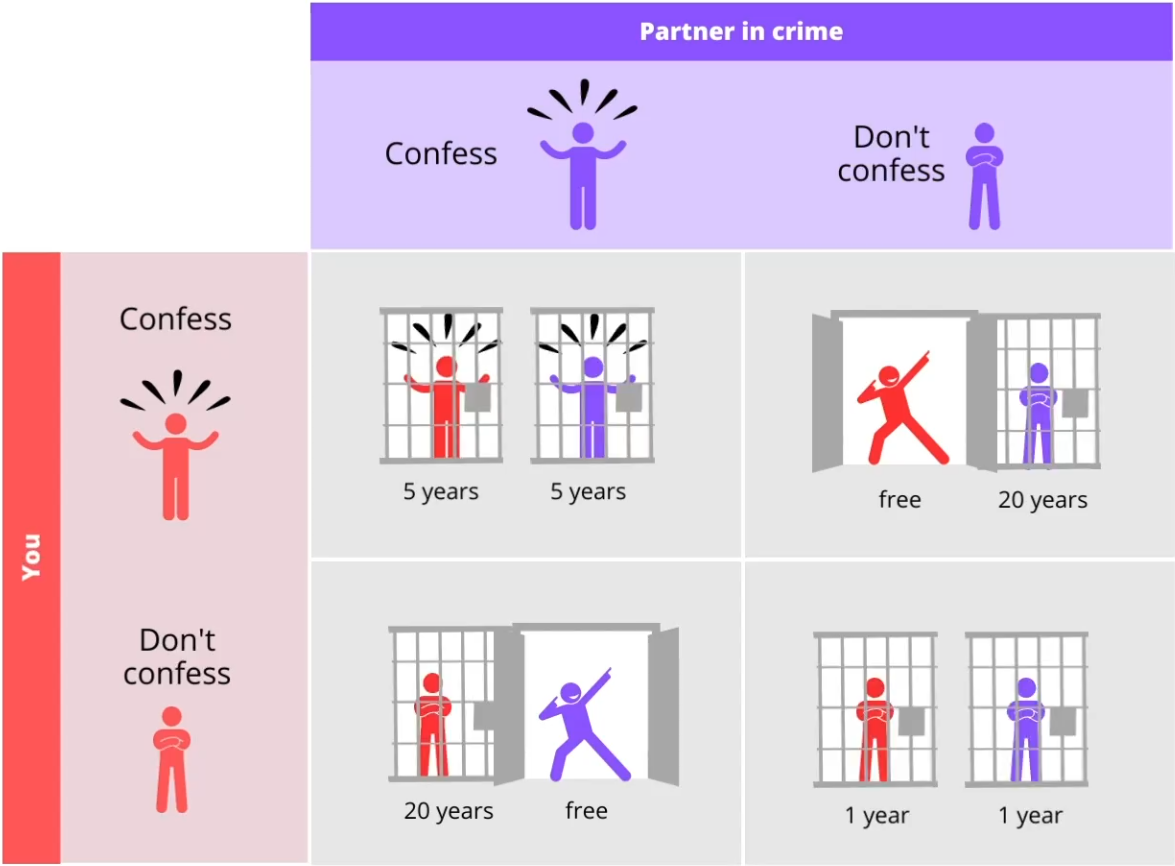
\includegraphics[width=0.7\linewidth]{../images/12-prisoners-dilemma.png}
				\caption{depictions of the outcomes for the prisoner dilemma}
				\label{fig:12-prisoners-dilemma}
			\end{figure}
			What must one do when faced with this situation? It really depends on what your partner does. But in general it is better to confess, this minimizes the chance of you going to prison for a long time. On the other hand, not confessing would lead to the minimal amount of jail time between them. \\
			\\
			In the prisoner dilemma, the participants are not anonymous, they each bare a large responsibility towards the outcome of the situation. When talking about climate change and meat consumption, this is not the case. There are many parties involved which makes it completely different. \\
			\\
			\newpage
			Going back to the card experiment we can now find some meaning in a social dilemma. Going with the green card is called a \textbf{cooperative choice}, while the blue pick would be called a \textbf{competitive choice}.  A number of factors have been experimentally shown to have an effect on the results:
			\begin{enumerate}
				\item It is important that people thoroughly realize the mutual dependence in the situation. This grows when consecutive choices have to be made with feedback about the results after every choice. Awareness of the impact one has is very important. 
				\item The number of parties involved in the dilemma affects cooperation. The more participants, the more competitive choices will be made. This is because people try to ride free on the cooperative choices others make. 
				\item Communication promotes cooperation. 
				\item Cooperation decreases when the choices are made by groups instead of individuals. This is because a sort of `us' vs `them' mentality crops up. 
				\item Competition decreases when individual choices are more visible. This is because nobody wants to be perceived as the bad guy who ruins it for the rest.
				\item Research points to important individual differences among types of participants
			\end{enumerate}
		\newpage
		\subsection{Individual differences}
			The research for individual differences is mainly based on three types of studies: publicly  available information, experimental research and questionnaires. \\
			\\
			The \textbf{New Ecological Paradigm}  by Riley Dunlap is an example of such a questionnaire. It states a number of prompts and asks the participant to rate the extent in which they agree with them. It is shown to be a reliable and accurate  way to gain insight into opinions and behavioural intentions. The results of the questionnaire about climate show the following interesting correlations:
			\begin{description}
				\item[Relevant knowledge] The more ecologically literate one is, the more inclined they will be to make more sustainable choices. 
				\item[personality traits] Research has identified five personality traits that describe a personality accurately. The latter three correlate well with environment-friendly behaviour:
				\begin{itemize}
					\item extroversion 
					\item neurotic-ism
					\item agreeableness
					\item openness
					\item conscientiousness				
				\end{itemize}
				\item[Gender] In general, women are more concerned about the environment and nature than men. 
				\item[Education and ocupation] Lower educated people are not as used to having an influence and being able to choose, so they are less attached to it. 
				\item[beliefs and values] In the USA, political affiliation is a better predictor of global warming-related behaviour than education and scientific knowledge. Furthermore, there is a strong correlation between religiousness and sustainable behaviour. 
				\item[Materialism] There is a negative correlation with materialistic people and climate.
				\item[External locus of control] people who attribute successes and failures to luck rather than their own effort display less sustainable behaviour than people with an internal locus of control.
			\end{description}
			
		\newpage	
		\subsection{Thoughtful or automatic}
			The human mind has long been thought of as rational, and economically conscious. This was extended to thinking that if we provide the right information about sustainability, people would take action for the better. \\
			\\
			This, of course, is not true. \textbf{Daniel Kahneman} makes the distinction in his book \textbf{Thinking Fast and Slow} between \textbf{two thought processes} or two systems. \textbf{System two} is the very rational process that we associate with the human mind, it is the second system because it is submissive to the first system. This \textbf{system one} is the dominant process and represents the unconscious thinking. System one is a lot more energy efficient since it happens unconsciously. They are very fast but tend to fly under the radar as we are not aware that we have this thought process. \\
			\\
			For example, watching a video is something handled  by system one. It does not take a lot of effort to process the visual and auditory information presented to you. Interpreting what is actually happening is a job left to system two, this takes a lot more effort. Another example is riding a bike, while learning, this task is handled by system two. As you make more progress and get comfortable with it, cycling gets handed over to system one which frees up system two to do other tasks. \\
			\\
			If something like riding a bike can be automated into a system one process, we can leave other complex tasks to the highly automated system one as well. For example communication is handled by system one as well. This means that a lot of information -- including sustainability -- flies under the radar when we don't actively process it with system two. \\
			\\
			Another sustainable example is the issue of rising energy prices. With purely rationally thinking brain, insulating your house is a no no-brainer.  However, this is a long term economical issue which flies under the radar with system one. This has a dramatical impact on the rate at which people insulate their homes. A solution for this problem is to incentivize people with subsidies, not only for the act of insulating but also for removing barriers to  insulate such as cleaning up the attic. 
			
		\subsection{Persuasive communication}
			Because we know people mostly process their thoughts unconsciously, we can assume this also applies to communication processes as well. \textbf{Predominant unconscious processing} means that the sender of a message will be using a lot of intuition when sending messages to others. The receiver will then use their own cognitive intuitions to process these messages. \\
			\\
			When a sender is invested in the message, they will consciously think about how to relay it in order to motivate a receiver. At the same time the receiver will have their own ideas and biasses about the message, influencing about how they act upon it. There are two types of messages processed by the receiver: \textbf{persuasion} and \textbf{rhetoric}. The former is what's going on on a day to day basis with hundreds or thousands of messages. The latter are messages which the receivers really think they should take time for. The difference between these two holds the key to behavioural change.\\
			\\
			If we want people to think differently and behave other than they are now, we have \textbf{two different sets of drivers to make that behavioural change}.
			\begin{description}
				\item[Conscious drivers] Legal restrictions, rhetoric campaigns... . Can influence conscious system two behaviour (only works if someone actually listens and pays attention)
				\item[Unconscious drivers] persuasion, the design of the situation that you are operating in... can influence unconscious, system one behaviour.   (change your mind little by little)
			\end{description}
			These changes should always be looked at in a combination, because it will always be more effective if both systems are aware and cooperating about the intended behavioural change.
			
		\subsection{Stakeholder system}
			With the knowledge of how people communicate as both sender and receiver. We should revisit the way in which we think about communication, where the sender sends a message to the receiver with a potential for noise to slip in as seen on figure \ref{fig:12-sender-receiver-model}. \\
			
			\begin{figure}[h]
				\centering
				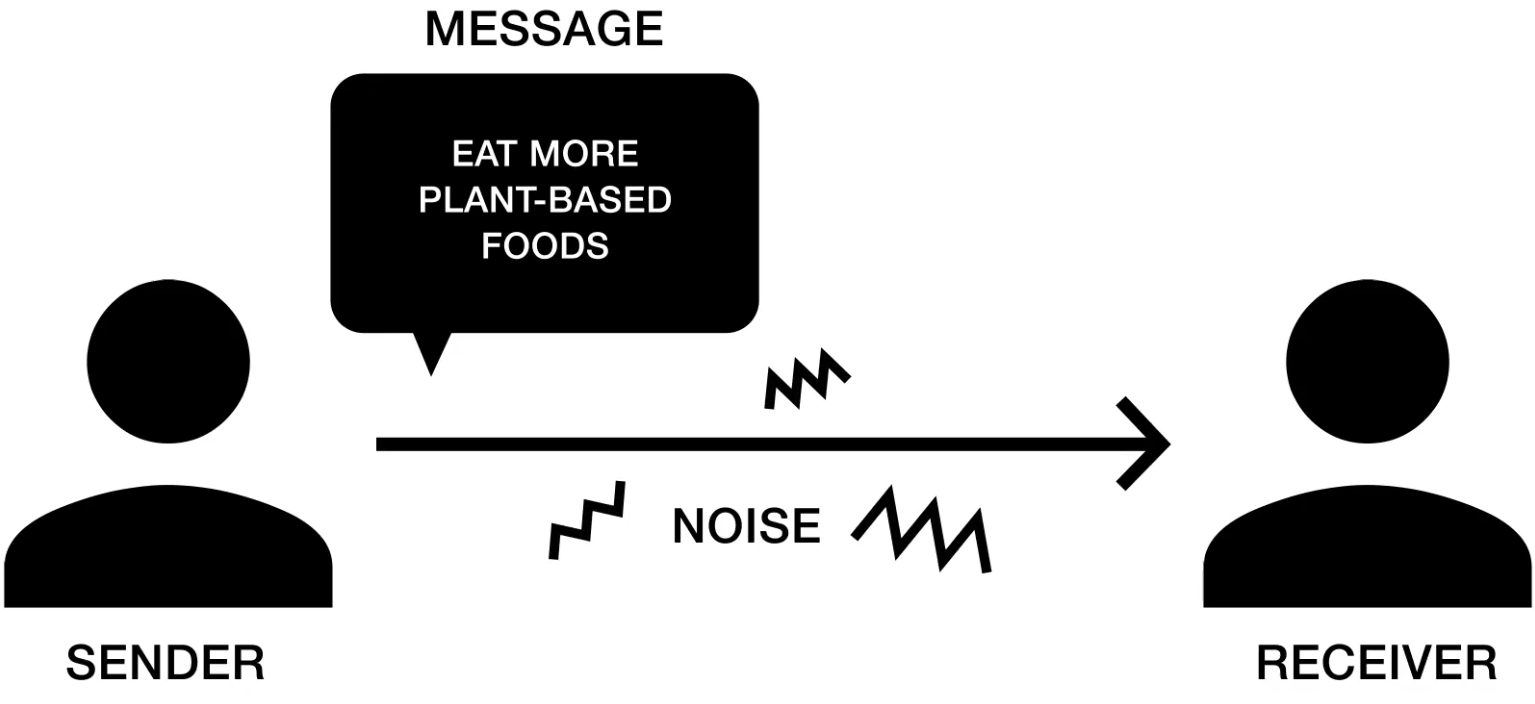
\includegraphics[width=0.7\linewidth]{../images/12-sender-receiver-model.png}
				\caption{Dated sender receiver model}
				\label{fig:12-sender-receiver-model}
			\end{figure}
			This however is not accurate because it doesn't take system one into account. We use it to kind of filter all the different messages we receive, which makes us not pay any real attention to a lot of the messages. We want to divide our communication time between a lot of different things. This means your message will just be one message in a whole range of them. It is thus important to understand that a receiver will probably not devote a lot of time to your particular message. \\
			\\
			It is much better to represent communication as a \textbf{stakeholder system} such as seen in figure \ref{fig:12-stakeholder-model}. \\
			
			\begin{figure}[h]
				\centering
				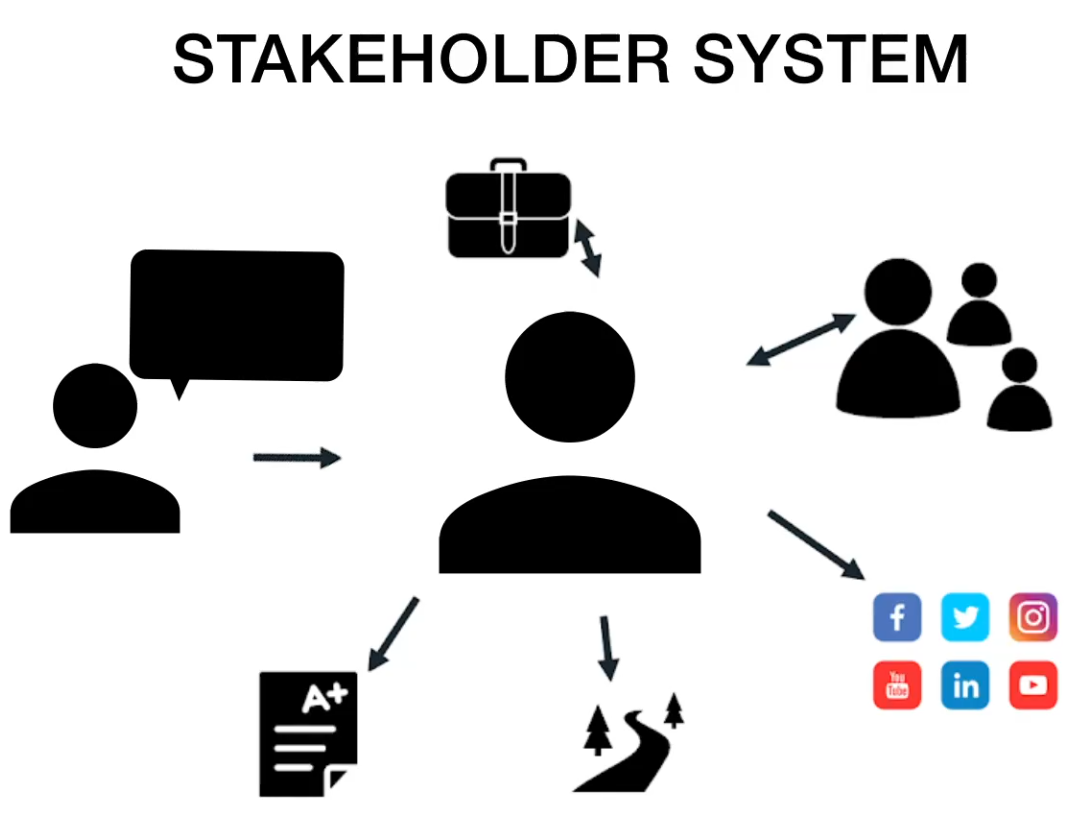
\includegraphics[width=0.7\linewidth]{../images/12-stakeholder-model.png}
				\caption{Stakeholder model}
				\label{fig:12-stakeholder-model}
			\end{figure}
			\newpage
			In this system there is one receiver with a lot of senders over different mediums. This means that there is a lot of competition between senders to get their message across to the receiver. It is important that every stakeholder gets a win for the system to work best. If the recipient wants a message, they go to a medium to accommodate this which is a win for the receiver. Vice versa, the medium wants recipients because otherwise it really isn't a medium any more. A medium also needs recipients to please advertisers which may be involved.  So the main stakes for the medium are to have recipients, but also senders and maybe advertisers that finance and at the same time also populate the medium.\\
			\\
			As a sender you want to reach recipients, often you will have to go through a medium for this. So your win is a cooperation with the medium and reaching out to recipients. Crafting a good message is thus not the only requirement, the choice of medium is also very important. 
			
		\subsection{Biases}
			\textbf{Biasses} are mental short-cuts that people take when they consider information and communication. They are important to take into account within the communication process. On the sender side, the illusion of attention and or communication with the receiver is a common one. \textbf{George Bernard Shaw} famously said that ``The single biggest problem with communication is the illusion that it has taken place''. When looking at this illusion we should not only think about the message as a whole but also the contents of that message. \\
			\\
			For instance, climate activists throwing a can of soup over a painting makes sure a lot of people see their message, but the content of their message is usually completely lost because of the way they  chose to convey their message.  So that's \textbf{a double layer of the illusion} of communication. And that double layer -- or that attention to the message, but not its content -- has also been demonstrated in a set of experimental studies. 
			
			\subsubsection{Norms}
				\textbf{Norms} are an incredibly persuasive driver in communication, we are influenced a lot by them. This can be explained by our tendency  to be influenced by a group because that helped our species survive and evolve into who we are now. There are essentially two types of norms we have to think about: (see figure \ref{fig:12-norm} as well)
				\begin{description}
					\item[Injunctive norms] These are norms which say what you should be doing to be accepted in a group. This is what we typically think of when we think of norms
					\item[Descriptive norms] These are the perceptions that we have about what others do or what we even just think they are doing. They might sometimes be in contrast with injunctive norms. 
				\end{description}
				
				\begin{figure}[h]
					\centering
					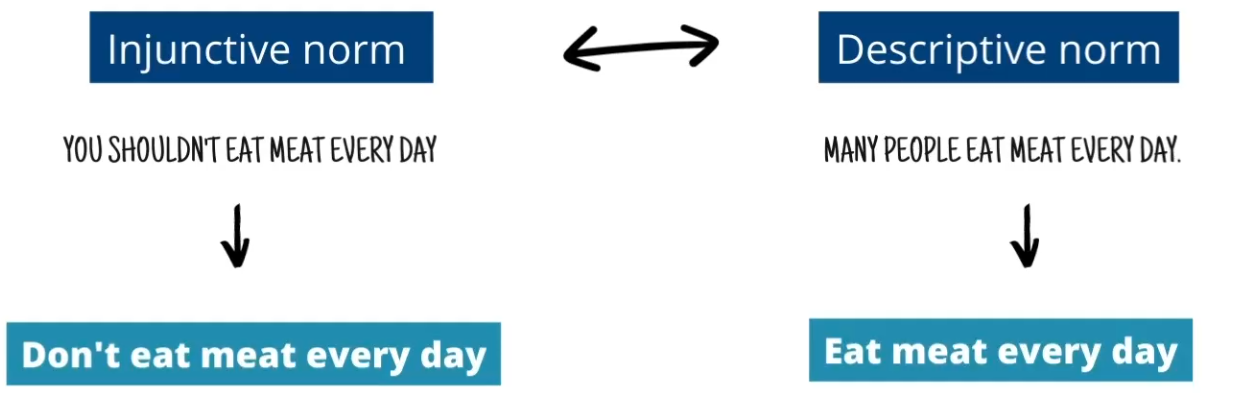
\includegraphics[width=0.7\linewidth]{../images/12-norm.png}
					\caption{Two different types of norms}
					\label{fig:12-norm}
				\end{figure}
				These norms work in opposite directions so they can have a large effect on the message you are trying to convey. To complicate matters more, the perception of those norms have an influence as well. It's perceptions of descriptive norms that are a very powerful driver and that are often neglected when we try to persuade other people.
				
			\subsubsection{Return on investment biases}
				When we put effort, time, energy or money into something, we usually do it to have a greater return at the end of the ride. There are a few biasses which have an effect on the way we think about these kinds of things. 
				\begin{description}
					\item[Sunk cost fallacy] This is when we let past investments influence future decisions. Instead, we should focus on current circumstances and make choices based on what makes sense now, regardless of previous expenses. For instance, replacing a relatively new car with a more suitable transport option is rational, even if it means letting go of the initial investment. The key is to prioritize present and future benefits over past costs.
					\item[Endownment effect] We tend to place higher value on things we already own or decisions we've made in the past. This is because we see them as part of our identity and life. Consequently, we often resist letting go of them, even when it might be more rational to do so.
					\item[Loss aversion] People avoid the psychological impact of loss and tend to value it more than a comparable gain. When communicating advice or instructions, it's essential to consider this aversion to loss and potentially reframe or rephrase suggestions accordingly.
					\item[Hyerpbolic discounting] This involves valuing immediate investments and returns more than those in the future. This bias influences decisions, making people favour immediate actions and rewards over delayed ones, even if the long-term benefits are significant.
				\end{description}
				In your communication, it's beneficial to minimize the perception of immediate investment and enhance the perception of immediate returns. This makes your message more persuasive, considering that people often have a return on investment mindset influenced by biases like sunk cost fallacy, loss aversion, endowment effect, and hyperbolic discounting.
			
\end{document}